\documentclass[11pt,a4paper]{report}
\usepackage[textwidth=37em,vmargin=30mm]{geometry}
\usepackage{calc,xunicode,amsmath,amssymb,paralist,enumitem,tabu,booktabs,datetime2,xeCJK,xeCJKfntef,listings}
\usepackage{tocloft,fancyhdr,tcolorbox,xcolor,graphicx,eso-pic,xltxtra,xelatexemoji}

\newcommand{\envyear}[0]{2025}
\newcommand{\envdatestr}[0]{2025-04-12}
\newcommand{\envfinaldir}[0]{webdb/2025/20250412/final}

\usepackage[hidelinks]{hyperref}
\hypersetup{
    colorlinks=false,
    pdfpagemode=FullScreen,
    pdftitle={Web Digest - \envdatestr}
}

\setlength{\cftbeforechapskip}{10pt}
\renewcommand{\cftchapfont}{\rmfamily\bfseries\large\raggedright}
\setlength{\cftbeforesecskip}{2pt}
\renewcommand{\cftsecfont}{\sffamily\small\raggedright}

\setdefaultleftmargin{2em}{2em}{1em}{1em}{1em}{1em}

\usepackage{xeCJK,xeCJKfntef}
\xeCJKsetup{PunctStyle=plain,RubberPunctSkip=false,CJKglue=\strut\hskip 0pt plus 0.1em minus 0.05em,CJKecglue=\strut\hskip 0.22em plus 0.2em}
\XeTeXlinebreaklocale "zh"
\XeTeXlinebreakskip = 0pt


\setmainfont{Brygada 1918}
\setromanfont{Brygada 1918}
\setsansfont{IBM Plex Sans}
\setmonofont{JetBrains Mono NL}
\setCJKmainfont{Noto Serif CJK SC}
\setCJKromanfont{Noto Serif CJK SC}
\setCJKsansfont{Noto Sans CJK SC}
\setCJKmonofont{Noto Sans CJK SC}

\setlength{\parindent}{0pt}
\setlength{\parskip}{8pt}
\linespread{1.15}

\lstset{
	basicstyle=\ttfamily\footnotesize,
	numbersep=5pt,
	backgroundcolor=\color{black!5},
	showspaces=false,
	showstringspaces=false,
	showtabs=false,
	tabsize=2,
	captionpos=b,
	breaklines=true,
	breakatwhitespace=true,
	breakautoindent=true,
	linewidth=\textwidth
}






\newcommand{\coverpic}[2]{
    % argv: itemurl, authorname
    Cover photo by #2~~(\href{#1}{#1})
}
\newcommand{\makeheader}[0]{
    \begin{titlepage}
        % \newgeometry{hmargin=15mm,tmargin=21mm,bmargin=12mm}
        \begin{center}
            
            \rmfamily\scshape
            \fontspec{BaskervilleF}
            \fontspec{Old Standard}
            \fontsize{59pt}{70pt}\selectfont
            WEB\hfill DIGEST
            
            \vfill
            % \vskip 30pt
            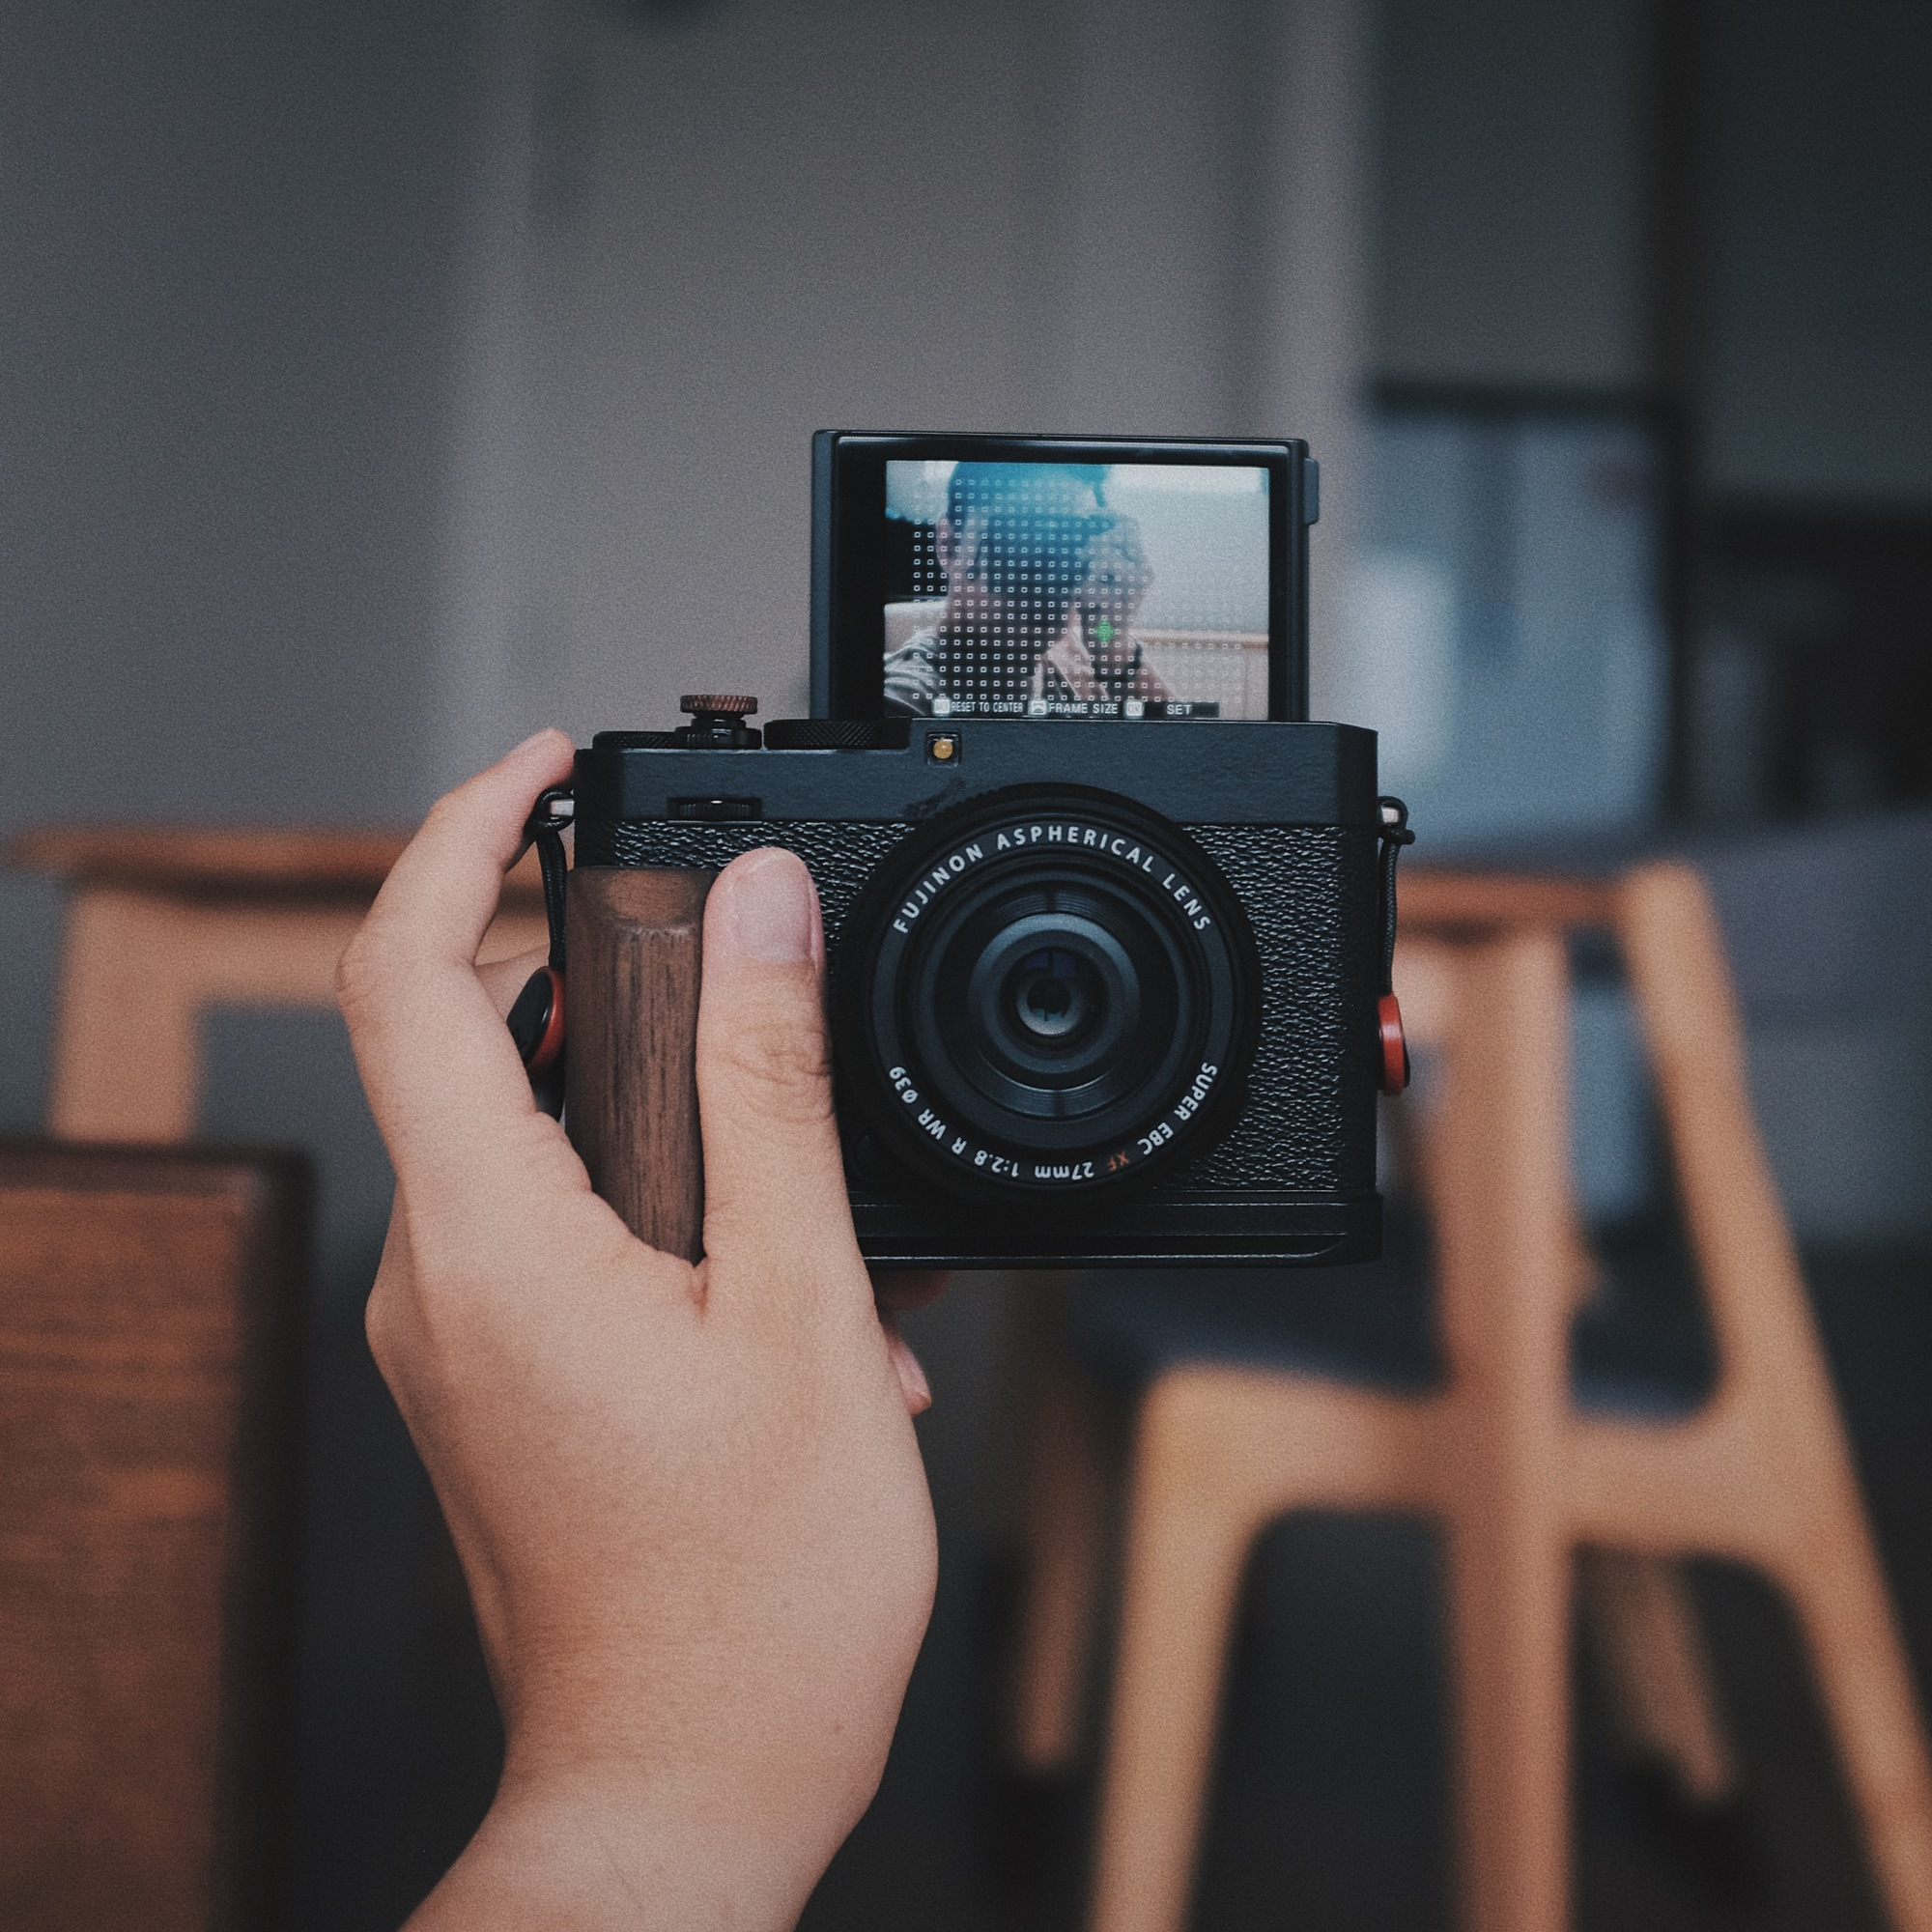
\includegraphics[width=\linewidth]{\envfinaldir/coverpic-prod.jpg}\par
            % \vskip 30pt
            \vfill

            \normalsize\rmfamily\scshape
            \copyright{} The Web Digest Project \hfill\large \envdatestr
        \end{center}
    \end{titlepage}
    % \restoregeometry
}
\newcommand{\simplehref}[1]{%
    \textcolor{blue!80!green}{\href{#1}{#1}}%
}
\renewcommand{\contentsname}{\center\Huge\sffamily\bfseries Contents\par\vskip 20pt}
\newcounter{ipartcounter}
\setcounter{ipartcounter}{0}
\newcommand{\ipart}[1]{
    % \vskip 20pt
    \clearpage
    \stepcounter{ipartcounter}
    \phantomsection
    \addcontentsline{toc}{chapter}{#1}
    % \begin{center}
    %     \Huge
    %     \sffamily\bfseries
    %     #1
    % \end{center}
    % \vskip 20pt plus 7pt
}
\newcounter{ichaptercounter}
\setcounter{ichaptercounter}{0}
\newcommand{\ichapter}[1]{
    % \vskip 20pt
    \clearpage
    \stepcounter{ichaptercounter}
    \phantomsection
    \addcontentsline{toc}{section}{\numberline{\arabic{ichaptercounter}}#1}
    \begin{center}
        \Huge
        \sffamily\bfseries
        #1
    \end{center}
    \vskip 20pt plus 7pt
}
\newcommand{\entrytitlefont}[1]{\subsection*{\raggedright\Large\sffamily\bfseries#1}}
\newcommand{\entryitemGeneric}[2]{
    % argv: title, url
    \parbox{\linewidth}{
        \entrytitlefont{#1}\par\vskip 5pt
        \footnotesize\ttfamily\mdseries
        \simplehref{#2}
    }\vskip 11pt plus 11pt minus 1pt
}
\newcommand{\entryitemGithub}[3]{
    % argv: title, url, desc
    \parbox{\linewidth}{
        \entrytitlefont{#1}\par\vskip 5pt
        \footnotesize\ttfamily\mdseries
        \simplehref{#2}\par\vskip 5pt
        \small\rmfamily\mdseries#3
    }\vskip 11pt plus 11pt minus 1pt
}
\newcommand{\entryitemAp}[3]{
    % argv: title, url, desc
    \parbox{\linewidth}{
        \entrytitlefont{#1}\par\vskip 5pt
        \footnotesize\ttfamily\mdseries
        \simplehref{#2}\par\vskip 5pt
        \small\rmfamily\mdseries#3
    }\vskip 11pt plus 11pt minus 1pt
}
\newcommand{\entryitemHackernews}[3]{
    % argv: title, hnurl, rawurl
    % \parbox{\linewidth}{
    %     \entrytitlefont{#1}\par\vskip 5pt
    %     \footnotesize\ttfamily\mdseries
    %     \simplehref{#3}\par
    %     \textcolor{black!50}{\href{#2}{#2}}
    % }\vskip 11pt plus 11pt minus 1pt
    \begin{minipage}{\linewidth}
            \entrytitlefont{#1}\par\vskip 5pt
            \footnotesize\ttfamily\mdseries
            \simplehref{#3}\par
            \textcolor{black!50}{\href{#2}{#2}}
    \end{minipage}\par\vskip 11pt plus 11pt minus 1pt
}







\begin{document}

\makeheader

\tableofcontents\clearpage




\ipart{Developers}
\ichapter{Hacker News}
\entryitemTwoLinks{Germany creates 'super–high-tech ministry' for research, technology, aerospace}{https://news.ycombinator.com/item?id=43658060}{https://www.science.org/content/article/germany-creates-super-high-tech-ministry-research-technology-and-aerospace}

\entryitemTwoLinks{Social Security Administration Moving Public Communications to X}{https://news.ycombinator.com/item?id=43657079}{https://www.wired.com/story/social-security-administration-regional-office-elon-musk-x/}

\entryitemTwoLinks{The PS3 Licked the Many Cookie}{https://news.ycombinator.com/item?id=43656279}{https://darkcephas.github.io/ps3\_failed/ps3\_failed.html}

\entryitemTwoLinks{Datastar: Web Framework for the Future?}{https://news.ycombinator.com/item?id=43655914}{https://chrismalek.me/posts/data-star-first-impressions/}

\entryitemTwoLinks{Leaked Meta data reveals campaign to remove pro-Palestine posts}{https://news.ycombinator.com/item?id=43655603}{https://www.dropsitenews.com/p/leaked-data-israeli-censorship-meta}

\entryitemTwoLinks{Erlang's not about lightweight processes and message passing (2023)}{https://news.ycombinator.com/item?id=43655221}{https://stevana.github.io/erlangs\_not\_about\_lightweight\_processes\_and\_message\_passing.html}

\entryitemTwoLinks{Bilinear interpolation on a quadrilateral using Barycentric coordinates}{https://news.ycombinator.com/item?id=43654912}{https://gpuopen.com/learn/bilinear-interpolation-quadrilateral-barycentric-coordinates/}

\entryitemTwoLinks{Rust CUDA Project}{https://news.ycombinator.com/item?id=43654881}{https://github.com/Rust-GPU/Rust-CUDA}

\entryitemTwoLinks{She Worked in a Harvard Lab to Reverse Aging, Until ICE Jailed Her}{https://news.ycombinator.com/item?id=43653998}{https://www.nytimes.com/2025/04/11/science/russian-scientist-ice-detained-harvard.html}

\entryitemTwoLinks{Adobe deletes Bluesky posts after backlash}{https://news.ycombinator.com/item?id=43653885}{https://petapixel.com/2025/04/10/adobe-deletes-bluesky-posts-after-furious-backlash/}

\entryitemTwoLinks{Fedora change aims for 99\% package reproducibility}{https://news.ycombinator.com/item?id=43653672}{https://lwn.net/Articles/1014979/}

\entryitemTwoLinks{Pentagon to terminate \$5.1B in IT contracts with Accenture, Deloitte}{https://news.ycombinator.com/item?id=43653004}{https://www.reuters.com/world/us/pentagon-terminate-51-billion-it-contracts-with-accenture-deloitte-others-2025-04-11/}

\entryitemTwoLinks{But what if I want a faster horse?}{https://news.ycombinator.com/item?id=43652723}{https://rakhim.exotext.com/but-what-if-i-really-want-a-faster-horse}

\entryitemTwoLinks{How to Make a Longbow}{https://news.ycombinator.com/item?id=43652160}{https://www.howtomakealongbow.co.uk}

\entryitemTwoLinks{Strengths Are Your Weaknesses}{https://news.ycombinator.com/item?id=43652024}{https://terriblesoftware.org/2025/03/31/your-strengths-are-your-weaknesses/}

\entryitemTwoLinks{Why I Program in Lisp}{https://news.ycombinator.com/item?id=43651576}{http://funcall.blogspot.com/2025/04/why-i-program-in-lisp.html}

\entryitemTwoLinks{Lead is still bad for your brain}{https://news.ycombinator.com/item?id=43651532}{https://neurofrontiers.blog/why-lead-is-still-bad-for-your-brain/}

\entryitemTwoLinks{The thing about Europe: it's the actual land of the free now}{https://news.ycombinator.com/item?id=43651489}{https://www.economist.com/europe/2025/04/10/the-thing-about-europe-its-the-actual-land-of-the-free-now}

\entryitemTwoLinks{Live Map of the London Underground}{https://news.ycombinator.com/item?id=43651390}{https://www.londonunderground.live/}

\entryitemTwoLinks{Playing in the Creek}{https://news.ycombinator.com/item?id=43650656}{https://www.hgreer.com/PlayingInTheCreek/}\ichapter{Phoronix}
\entryitemGeneric{\hskip 0pt{}AMD Releases ROCm 6.4 Without Any Official RDNA4 Support}{https://www.phoronix.com/news/AMD-ROCm-6.4-Released}

\entryitemGeneric{\hskip 0pt{}Running Linux 6.15 vs. 6.14 Performance With The AMD Ryzen AI 7 PRO 360}{https://www.phoronix.com/news/Linux-6.15-Ryzen-AI-7-PRO-360}

\entryitemGeneric{\hskip 0pt{}Intel Preps VRR Refactoring For Linux 6.16, More Xe3 Panther Lake Display Enablement}{https://www.phoronix.com/news/Intel-DRM-Next-Linux-6.16-1}

\entryitemGeneric{\hskip 0pt{}Ubuntu 25.04 vs. Fedora Workstation 42 Performance On AMD Strix Point}{https://www.phoronix.com/review/fedora-42-ubuntu-2504-zen5}

\entryitemGeneric{\hskip 0pt{}OpenVPN DCO Driver For The Linux Kernel Revised A 25th Time To Boost VPN Performance}{https://www.phoronix.com/news/OpenVPN-DCO-Linux-25th}

\entryitemGeneric{\hskip 0pt{}Linux 6.15 Fixes Intel Graphics Flickering Issue, Adds AMDGPU DMEM Cgroups Support}{https://www.phoronix.com/news/Linux-6.15-rc2-DRM-Fixes}

\entryitemGeneric{\hskip 0pt{}Haiku OS Continued Improving Hardware Driver Support In March}{https://www.phoronix.com/news/Haiku-OS-March-2025-Updates}

\entryitemGeneric{\hskip 0pt{}IBM z17 Open-Source Compiler Support Now Being Officially Recognized}{https://www.phoronix.com/news/IBM-z17-LLVM-Clang}

\entryitemGeneric{\hskip 0pt{}Linux 6.15 Lands Patches To Further Clean Up Its Spectre RSB Mitigations}{https://www.phoronix.com/news/Linux-6.15-x86-Fixes-RSB}\ichapter{Dribbble}
\entryitemGeneric{\hskip 0pt{}Nite Riot®\_Film Production // Case Study\_Vol.2.0}{https://dribbble.com/shots/25889874-Nite-Riot-Film-Production-Case-Study-Vol-2-0}

\entryitemGeneric{\hskip 0pt{}Lion}{https://dribbble.com/shots/25884438-Lion}

\entryitemGeneric{\hskip 0pt{}Fintech Web Design \& Landing Page for Puzzle}{https://dribbble.com/shots/25652139-Fintech-Web-Design-Landing-Page-for-Puzzle}

\entryitemGeneric{\hskip 0pt{}Web Design Crypto Trading}{https://dribbble.com/shots/25879747-Web-Design-Crypto-Trading}

\entryitemGeneric{\hskip 0pt{}Monster Pony Wooden toy}{https://dribbble.com/shots/25880300-Monster-Pony-Wooden-toy}

\entryitemGeneric{\hskip 0pt{}Educate AI Logo Design - Letter E, Monogram, Education}{https://dribbble.com/shots/25879659-Educate-AI-Logo-Design-Letter-E-Monogram-Education}

\entryitemGeneric{\hskip 0pt{}Hawkridge}{https://dribbble.com/shots/25877367-Hawkridge}

\entryitemGeneric{\hskip 0pt{}UI Design for Cargo Delivery Company}{https://dribbble.com/shots/25874804-UI-Design-for-Cargo-Delivery-Company}

\entryitemGeneric{\hskip 0pt{}Nite Riot®\_Film Production // Case Study\_Vol.1.0}{https://dribbble.com/shots/25874978-Nite-Riot-Film-Production-Case-Study-Vol-1-0}

\entryitemGeneric{\hskip 0pt{}UltraSlot}{https://dribbble.com/shots/25875506-UltraSlot}

\entryitemGeneric{\hskip 0pt{}Sidekick Ai 3d mascot}{https://dribbble.com/shots/25874949-Sidekick-Ai-3d-mascot}

\entryitemGeneric{\hskip 0pt{}🔐 Cybersecurity App Landing}{https://dribbble.com/shots/25873133--Cybersecurity-App-Landing}

\entryitemGeneric{\hskip 0pt{}Equati}{https://dribbble.com/shots/25858079-Equati}

\entryitemGeneric{\hskip 0pt{}Taiwan Travel Poster}{https://dribbble.com/shots/25877695-Taiwan-Travel-Poster}

\entryitemGeneric{\hskip 0pt{}Howzit}{https://dribbble.com/shots/25871668-Howzit}

\entryitemGeneric{\hskip 0pt{}Brainstorm}{https://dribbble.com/shots/25871145-Brainstorm}

\entryitemGeneric{\hskip 0pt{}Boxplates}{https://dribbble.com/shots/25869902-Boxplates}

\entryitemGeneric{\hskip 0pt{}Spark illustrations}{https://dribbble.com/shots/25872229-Spark-illustrations}

\entryitemGeneric{\hskip 0pt{}Nord Print Logo Design - Northern Star, Paper, Print, Printing}{https://dribbble.com/shots/25867726-Nord-Print-Logo-Design-Northern-Star-Paper-Print-Printing}

\entryitemGeneric{\hskip 0pt{}Medieval H}{https://dribbble.com/shots/25862061-Medieval-H}

\entryitemGeneric{\hskip 0pt{}Peach Media Logo Design}{https://dribbble.com/shots/25869696-Peach-Media-Logo-Design}

\entryitemGeneric{\hskip 0pt{}Quill Pen mark}{https://dribbble.com/shots/25871430-Quill-Pen-mark}

\entryitemGeneric{\hskip 0pt{}Skype Logo Redesign Concept}{https://dribbble.com/shots/25869984-Skype-Logo-Redesign-Concept}

\entryitemGeneric{\hskip 0pt{}Crypto Mobile App}{https://dribbble.com/shots/25869253-Crypto-Mobile-App}


\ipart{Developers~~~~(zh-Hans)}
\ichapter{Solidot}
\entryitemGeneric{\hskip 0pt{}英特尔 CPU 可能受中国对美关税政策影响}{https://www.solidot.org/story?sid=81023}

\entryitemGeneric{\hskip 0pt{}任天堂将越南制造的 Switch 2 游戏机几乎全部出口到美国}{https://www.solidot.org/story?sid=81022}

\entryitemGeneric{\hskip 0pt{}2024 年 58\% 的 PC 游戏收入来自微交易}{https://www.solidot.org/story?sid=81021}

\entryitemGeneric{\hskip 0pt{}科学家测量出中微子至今最精确质量上限 0.45 eV }{https://www.solidot.org/story?sid=81020}

\entryitemGeneric{\hskip 0pt{}美国政治措辞日益倾向于个人信念而不是事实}{https://www.solidot.org/story?sid=81019}

\entryitemGeneric{\hskip 0pt{}小鼠研究发现淀粉基微塑料可能存在健康风险}{https://www.solidot.org/story?sid=81018}

\entryitemGeneric{\hskip 0pt{}美国不想要孩子的人数在增长}{https://www.solidot.org/story?sid=81017}

\entryitemGeneric{\hskip 0pt{}Switch 2 推迟在华发售}{https://www.solidot.org/story?sid=81016}

\entryitemGeneric{\hskip 0pt{}美国暂停对等关税 90 天,对华关税提高到 125\%}{https://www.solidot.org/story?sid=81015}

\entryitemGeneric{\hskip 0pt{}科学家公布迄今最详尽的哺乳动物大脑连接图谱}{https://www.solidot.org/story?sid=81014}

\entryitemGeneric{\hskip 0pt{}Google 宣布了第七代 TPU 处理器 Ironwood}{https://www.solidot.org/story?sid=81013}

\entryitemGeneric{\hskip 0pt{}加固 Firefox 前端}{https://www.solidot.org/story?sid=81012}

\entryitemGeneric{\hskip 0pt{}OpenSSH 10.0 释出}{https://www.solidot.org/story?sid=81011}

\entryitemGeneric{\hskip 0pt{}中国将美国商品关税提高到 84\%}{https://www.solidot.org/story?sid=81010}

\entryitemGeneric{\hskip 0pt{}无权者不喜欢看公正中立的新闻}{https://www.solidot.org/story?sid=81009}

\entryitemGeneric{\hskip 0pt{}日本小镇流行大叔集卡游戏}{https://www.solidot.org/story?sid=81008}

\entryitemGeneric{\hskip 0pt{}Git 诞生二十周年}{https://www.solidot.org/story?sid=81007}

\entryitemGeneric{\hskip 0pt{}IBM 宣布 z17 大型机}{https://www.solidot.org/story?sid=81006}

\entryitemGeneric{\hskip 0pt{}科学家分离出候选最苦物质}{https://www.solidot.org/story?sid=81005}

\entryitemGeneric{\hskip 0pt{}黑客利用 Windows 0day 攻击美国 IT 和房地产公司}{https://www.solidot.org/story?sid=81004}\ichapter{V2EX}
\entryitemGeneric{\hskip 0pt{}[职场话题] 基层足球教练员,工作上有些迷茫,欢迎大家给些建议}{https://www.v2ex.com/t/1124900}

\entryitemGeneric{\hskip 0pt{}[问与答] 为啥一个私企还有吃大锅饭的呢 [吐槽]}{https://www.v2ex.com/t/1124899}

\entryitemGeneric{\hskip 0pt{}[生活] 最好的生活是适合自己的生活}{https://www.v2ex.com/t/1124898}

\entryitemGeneric{\hskip 0pt{}[职场话题] 这次的面试让我怀疑——我是不是被瞧不起了?}{https://www.v2ex.com/t/1124897}

\entryitemGeneric{\hskip 0pt{}[JetBrains] JetBrains 旗下的 Fleet ide 有人用过吗?使用体验怎么样?}{https://www.v2ex.com/t/1124896}

\entryitemGeneric{\hskip 0pt{}[程序员] 换个花样发个口令红包}{https://www.v2ex.com/t/1124893}

\entryitemGeneric{\hskip 0pt{}[京东] 为什么我的京东账号被强行设置了新版详情页,难用的一}{https://www.v2ex.com/t/1124892}

\entryitemGeneric{\hskip 0pt{}[PostgreSQL] PostgreSQL 通过分 Database 做多租户可行吗? PostgreSQL 多租户的正确姿势}{https://www.v2ex.com/t/1124891}

\entryitemGeneric{\hskip 0pt{}[生活] 自行车通勤一年的感想}{https://www.v2ex.com/t/1124890}

\entryitemGeneric{\hskip 0pt{}[问与答] 大佬们用 iOS Loon 代理工具你们都用谁的配置规则呀?}{https://www.v2ex.com/t/1124889}

\entryitemGeneric{\hskip 0pt{}[求职] [求职] 做过 Database/Bigdata/Cloud/Infra,想投 AI Infra / 系统工程方向}{https://www.v2ex.com/t/1124888}

\entryitemGeneric{\hskip 0pt{}[问与答] 为什么 2025 年了安卓还是做的这么糙,这真的是很难解的问题吗?}{https://www.v2ex.com/t/1124886}

\entryitemGeneric{\hskip 0pt{}[问与答] 求推荐 iOS 的语音输入法?}{https://www.v2ex.com/t/1124884}

\entryitemGeneric{\hskip 0pt{}[分享发现] Google A2A 尝试}{https://www.v2ex.com/t/1124883}

\entryitemGeneric{\hskip 0pt{}[YouTube] YouTube 去广告哪个插件好用?}{https://www.v2ex.com/t/1124881}

\entryitemGeneric{\hskip 0pt{}[汽车] 求助:小米 su7 与沃尔沃 s60 如何选择}{https://www.v2ex.com/t/1124880}

\entryitemGeneric{\hskip 0pt{}[Telegram] 电报账号 登录}{https://www.v2ex.com/t/1124879}

\entryitemGeneric{\hskip 0pt{}[职场话题] 高层不让现在的领导管某个项目说明什么}{https://www.v2ex.com/t/1124878}

\entryitemGeneric{\hskip 0pt{}[Windows] Win 下 Edge 不支持 hvec 视频}{https://www.v2ex.com/t/1124876}

\entryitemGeneric{\hskip 0pt{}[分享创造] Radarr 和 Sonarr 的海报上可以显示豆瓣评分了}{https://www.v2ex.com/t/1124875}

\entryitemGeneric{\hskip 0pt{}[分享创造] 内测邀请 | 我做了一个用 AI 给老年人写回忆录的小程序}{https://www.v2ex.com/t/1124874}

\entryitemGeneric{\hskip 0pt{}[职场话题] 即将被安排转岗,下车间炼铁,不想去怎么办}{https://www.v2ex.com/t/1124873}

\entryitemGeneric{\hskip 0pt{}[中州韻] 小狼毫的输入法工具栏如何关掉?}{https://www.v2ex.com/t/1124872}

\entryitemGeneric{\hskip 0pt{}[问与答] electron 下载限速}{https://www.v2ex.com/t/1124871}

\entryitemGeneric{\hskip 0pt{}[Tesla] 关于动能回收舆情的一些疑惑}{https://www.v2ex.com/t/1124870}

\entryitemGeneric{\hskip 0pt{}[开源软件] 推荐一下 conda 生态的新包管理 pixi}{https://www.v2ex.com/t/1124869}

\entryitemGeneric{\hskip 0pt{}[问与答] infuse 现在搭配哪个网盘比较好用?}{https://www.v2ex.com/t/1124868}

\entryitemGeneric{\hskip 0pt{}[生活] 患有罕见病,医生都不敢给我开中成药…}{https://www.v2ex.com/t/1124867}

\entryitemGeneric{\hskip 0pt{}[投资] 如果坚定的看空美国,那么做什么能够获利呢?}{https://www.v2ex.com/t/1124866}

\entryitemGeneric{\hskip 0pt{}[问与答] 用小米手机的朋友,你们是怎么备份私密相册的?}{https://www.v2ex.com/t/1124864}

\entryitemGeneric{\hskip 0pt{}[投资] 买黄金理财,选择银行的积存金还是基金的黄金 etf?}{https://www.v2ex.com/t/1124862}

\entryitemGeneric{\hskip 0pt{}[职场话题] 华为内部转岗两个方向请各位大佬给个建议}{https://www.v2ex.com/t/1124861}

\entryitemGeneric{\hskip 0pt{}[程序员] 大家平时用 Cursor 的时候,遇到最多的问题是什么?}{https://www.v2ex.com/t/1124858}

\entryitemGeneric{\hskip 0pt{}[Apple] 如何将 FaceTime(视频通话)联系人放在手机桌面上}{https://www.v2ex.com/t/1124857}

\entryitemGeneric{\hskip 0pt{}[MacBook] 买 mac 还是 windows}{https://www.v2ex.com/t/1124856}

\entryitemGeneric{\hskip 0pt{}[OpenAI] 你们在用 Mac 版 ChatGPT 时,有遇到快捷键失效或输入内容自动消失的情况吗?}{https://www.v2ex.com/t/1124855}

\entryitemGeneric{\hskip 0pt{}[分享创造] 跟风做 AI Coding Agent : Deepseek v3 新模型审美很到位!生成小游戏也很猛!送免费额度}{https://www.v2ex.com/t/1124854}

\entryitemGeneric{\hskip 0pt{}[随想] 聊天是一门技能}{https://www.v2ex.com/t/1124853}

\entryitemGeneric{\hskip 0pt{}[深圳] 羽毛球球搭子,有没有的!}{https://www.v2ex.com/t/1124851}

\entryitemGeneric{\hskip 0pt{}[V2EX] Clion 的 copilot 崩了。}{https://www.v2ex.com/t/1124850}

\entryitemGeneric{\hskip 0pt{}[问与答] B 站网页版推荐区总有恶心的广告伪装成正常视频,有啥办法过滤一下吗?}{https://www.v2ex.com/t/1124849}

\entryitemGeneric{\hskip 0pt{}[分享发现] 使用 tauri2.0 打包了个 json 解析工具}{https://www.v2ex.com/t/1124848}

\entryitemGeneric{\hskip 0pt{}[分享创造] 基于 GPT-4o 的各种场景图片的聚合生成网站}{https://www.v2ex.com/t/1124847}

\entryitemGeneric{\hskip 0pt{}[VPS] 有啥便宜的 vps 没有封锁 googlevideo.com}{https://www.v2ex.com/t/1124846}

\entryitemGeneric{\hskip 0pt{}[程序员] 今天 rubygems 缓存不更新}{https://www.v2ex.com/t/1124845}

\entryitemGeneric{\hskip 0pt{}[问与答] Windows 程序 EV 证书怎么整?}{https://www.v2ex.com/t/1124844}

\entryitemGeneric{\hskip 0pt{}[问与答] Trae 把我 48g Mac 干死机这件事}{https://www.v2ex.com/t/1124842}

\entryitemGeneric{\hskip 0pt{}[Spotify] 分享一个菲律宾 Spotify 开通教程 需要支持 eSIM 功能}{https://www.v2ex.com/t/1124841}

\entryitemGeneric{\hskip 0pt{}[分享发现] 英语的月份好不合理,今天终于找到原因了。}{https://www.v2ex.com/t/1124840}

\entryitemGeneric{\hskip 0pt{}[macOS] mac 15.4 系统国行还能启用 Apple AI 吗}{https://www.v2ex.com/t/1124839}


\ipart{Generic News}
\ichapter{AP News}
\entryitemWithDescription{\hskip 0pt{}US Attorney Habba investigating New Jersey governor over immigration enforcement policy}{https://apnews.com/article/dbf95a1dc06aa35270b6c6f591e0c31c}{}

\entryitemWithDescription{\hskip 0pt{}Eric Dane, star of `Euphoria' and `Grey's Anatomy,' reveals he has ALS}{https://apnews.com/article/a55253de0ba9eebf7335915f31c5d066}{}

\entryitemWithDescription{\hskip 0pt{}Australian woman unknowingly gives birth to a stranger's baby after IVF clinic error}{https://apnews.com/article/e587580649843d33f67b46afc5f30767}{}

\entryitemWithDescription{\hskip 0pt{}Cabot Creamery butter recalled over fecal bacteria contamination}{https://apnews.com/article/1badb501647b83790f5ebdf9eb82b2f0}{}

\entryitemWithDescription{\hskip 0pt{}Prada agrees to buy rival fashion house Versace in a deal valued at \$1.4 billion}{https://apnews.com/article/9bef87f68bd80f00d379d4b3628f60ad}{}

\entryitemWithDescription{\hskip 0pt{}An American pastor was abducted at gunpoint in South Africa while preaching a sermon}{https://apnews.com/article/2ab7330c428838e917f60e54bf64c962}{}

\entryitemWithDescription{\hskip 0pt{}Influencer Andrew Tate accused of pointing gun at woman's face ahead of London civil case}{https://apnews.com/article/136b75eb0ff2b3e0c299c27de1276664}{}

\entryitemWithDescription{\hskip 0pt{}A machine using ultrasound and AI can gauge the fattiness of a tuna fish}{https://apnews.com/article/b17bc843735a79cafb9a89033afaa578}{}

\entryitemWithDescription{\hskip 0pt{}Masters whiz kid: Jose Luis Ballester takes a different kind of relief and does No. 1 at No. 13}{https://apnews.com/article/09a133c9218e388d43a71b5ff9abd105}{}

\entryitemWithDescription{\hskip 0pt{}Pronouns in some reporters' email signatures get a stony response from Trump administration}{https://apnews.com/article/7cec13e2872bb07459bc3a630160577d}{}

\entryitemWithDescription{\hskip 0pt{}Mega Millions tickets rise to \$5 but lottery promises more giant jackpots}{https://apnews.com/article/900bf62127057b4124d8302f3200497a}{}

\entryitemWithDescription{\hskip 0pt{}Pope makes surprise appearance at St. Peter's Square, 2 weeks after leaving hospital}{https://apnews.com/article/50973c32de3f6e2cc1fd9dc036968f70}{}

\entryitemWithDescription{\hskip 0pt{}We got a behind-the-scenes look at Nintendo Switch 2. These are our thoughts}{https://apnews.com/article/63b0e49951ed09a9532ca55b4b35002e}{}






\clearpage
\leavevmode\vfill
\footnotesize

Copyright \copyright{} 2023-2025 Neruthes and other contributors.

This document is published with CC BY-NC-ND 4.0 license.

The entries listed in this newsletter may be copyrighted by their respective creators.

This newsletter is generated by the Web Digest project.

The newsletters are also delivered via Telegram channel \CJKunderline{\href{https://t.me/webdigestchannel}{https://t.me/webdigestchannel}}.\\
RSS feed is available at \CJKunderline{\href{https://webdigest.pages.dev/rss.xml}{https://webdigest.pages.dev/rss.xml}}.

This newsletter is available in PDF at
\CJKunderline{\href{https://webdigest.pages.dev/}{https://webdigest.pages.dev/}}.

The source code being used to generate this newsletter is available at\\
\CJKunderline{\href{https://github.com/neruthes/webdigest}{https://github.com/neruthes/webdigest}}.

This newsletter is also available in
\CJKunderline{\href{http://webdigest.pages.dev/readhtml/\envyear/WebDigest-20250412.html}{HTML}} and
\CJKunderline{\href{https://github.com/neruthes/webdigest/blob/master/markdown/\envyear/WebDigest-20250412.md}{Markdown}}.


\coverpic{https://unsplash.com/photos/a-car-driving-down-a-dirt-road-in-the-desert-nD0OAJzt43U}{Willian Justen de Vasconcellos}


\end{document}
